{
% \let\cleardoublepage\relax % you can use this command to disable \cleardoublepage

\chapter{LaTeX使用说明}\label{chap:chapter1}
{
章引,本章主要分析XXXX.

\section{图表使用}

插入 pdf 图片,如图 \ref{fig:figure1} 所示.
\begin{figure}[!htbp]
    \centering
    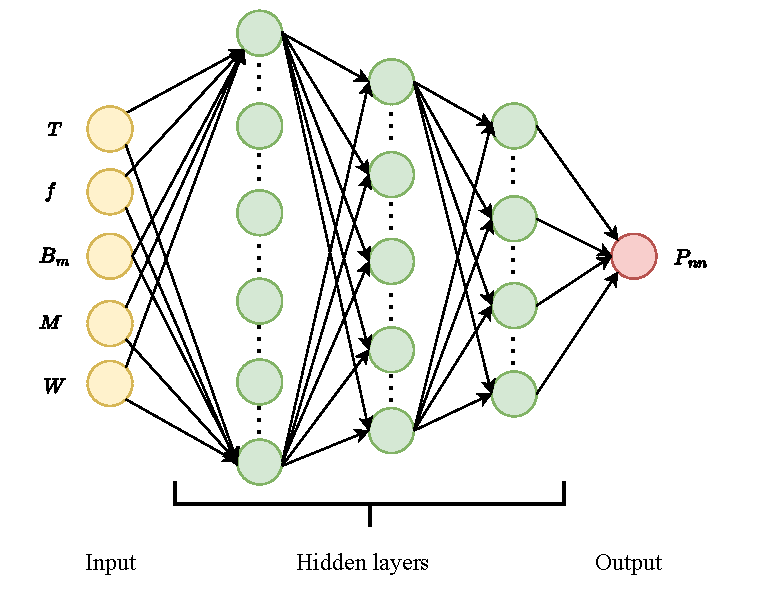
\includegraphics[width=0.40\textwidth]{figure1}
    \caption{插入 pdf 图片.}
    % \bicaption{\enspace 样图}{\enspace Sample Figure}
    % \fignote{对图片的注释}
    \label{fig:figure1}
\end{figure}

插入 png 图片,如图 \ref{fig:figure2} 所示.
\begin{figure}[!htbp]
    \centering
    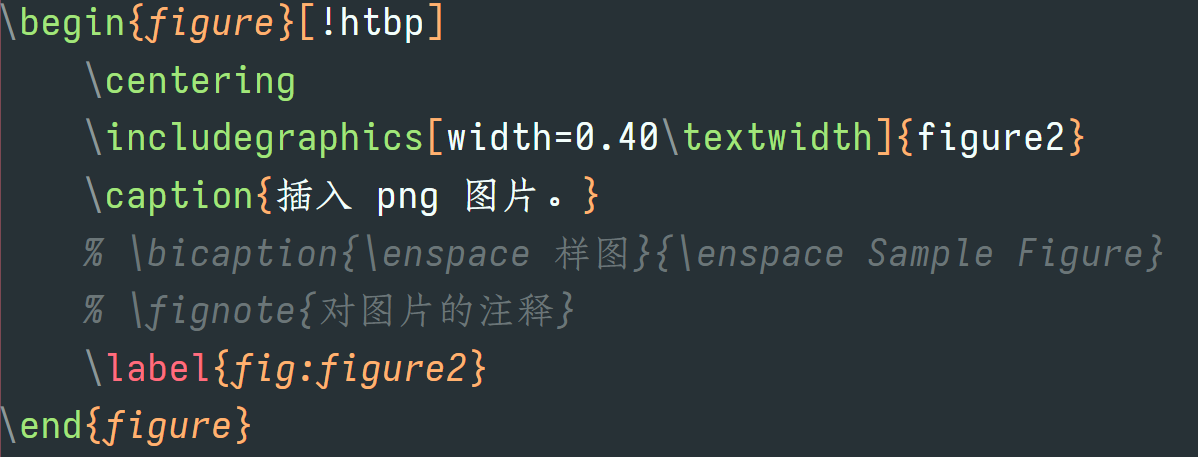
\includegraphics[width=0.40\textwidth]{figure2}
    \caption{插入 png 图片.}
    % \bicaption{\enspace 样图}{\enspace Sample Figure}
    % \fignote{对图片的注释}
    \label{fig:figure2}
\end{figure}

三线表设置,如表 \ref{tab:table1} 所示.
\begin{table}[!htbp]
    % \bicaption{\enspace 这是一个样表}{\enspace This is a sample table}
    \caption{插入三线表,表中字号设置为 \textbf{\backslash footnotesize}, 默认为 5 号字.}
    \label{tab:table1}
    \centering
    \footnotesize% fontsize
    \setlength{\tabcolsep}{4pt}% column separation
    % \renewcommand{\arraystretch}{1.2}%row space 
    \begin{tabular}{lcccccccc}
        \toprule
        行号 & \multicolumn{8}{c}{跨多列的标题}\\
        %\cline{2-9}% partial hline from column i to column j
        \midrule
        Row 1 & $1$ & $2$ & $3$ & $4$ & $5$ & $6$ & $7$ & $8$\\
        Row 2 & $1$ & $2$ & $3$ & $4$ & $5$ & $6$ & $7$ & $8$\\
        Row 3 & $1$ & $2$ & $3$ & $4$ & $5$ & $6$ & $7$ & $8$\\
        Row 4 & $1$ & $2$ & $3$ & $4$ & $5$ & $6$ & $7$ & $8$\\
        \bottomrule
    \end{tabular}
\end{table}

有序列表:
\begin{enumerate}
    \item item1.
    \item item2.
\end{enumerate}

无序列表:
\begin{itemize}
    \item item1.
    \item item2.
\end{itemize}

公式:
\begin{equation}
    \boldsymbol{y} = f(\boldsymbol{x}) + \boldsymbol{\varepsilon}, \boldsymbol{x}\in\mathbb{R}^n, \label{eq:equation1}
\end{equation}
见式~\eqref{eq:equation1}.

参考文献引用格式\cite{journal, inproceedings, book}.

\vspace*{2cm}
{\colorbox[rgb]{0.9,0.6,0.2}{本模板根据中国科学院大学模板修改得到,具体可查看此链接:}}

{\colorbox[rgb]{0.9,0.6,0.2}{\href{https://github.com/mohuangrui/ucasthesis}{https://github.com/mohuangrui/ucasthesis}.}}


}
}
